\documentclass{article}
\usepackage{ctex}
\usepackage{bm}
\usepackage{enumitem}
\usepackage{mathrsfs}
\usepackage{subcaption}
\usepackage{amsmath,amsthm,amsfonts,amssymb}
\usepackage{iidef}
\DeclareMathOperator{\sinc}{sinc}
\DeclareMathOperator{\rect}{rect}
\newtheorem{definition}{定义}
\newtheorem{thm}{定理}
\newtheorem{pro}{命题}
\newtheorem{cor}{推论}
\thecourseinstitute{清华大学深圳研究生院}
\thecoursename{统计信号处理}
\theterm{2018年春季学期}
\hwname{课后习题}
\slname{\heiti{解}}
\begin{document}
\courseheader
\name{赵丰}


\begin{enumerate}
\item 试推导如下情况的似然比。
\begin{align*}
H_0 & :  z\sim N(m_0,\sigma_0^2) \\
H_1 & :  z\sim N(m_1,\sigma_1^2)
\end{align*}
并求判决域和错误概率。
\begin{solution}
\begin{align}
\lambda(z) = & \frac{p(z|H_1)}{p(z|H_0)} \\
            = & \frac{\sigma_0}{\sigma_1}\exp(-\frac{(z-m_1)^2}{2\sigma_1^2}+\frac{(z-m_0)^2}{2\sigma_0^2})\label{eq:Gaussian_likelyhood_ratio}
\end{align}
\begin{align*}
\mathcal{Z}_0 = & \{z|\lambda(z) < \lambda_B\} \\
\mathcal{Z}_1 = & \{z|\lambda(z) > \lambda_B\}
\end{align*}
\begin{align*}
P_F = P(D_1,H_0) = & \int_{z\in \mathcal{Z}_1} p(z|H_0)dz \\
P_M = P(D_0,H_1) = & \int_{z\in \mathcal{Z}_0} p(z|H_1)dz 
\end{align*}
\end{solution}
\item 考虑一二元对称信道,$\epsilon$是交叉概率(假定$\epsilon< \frac{1}{2}$),即信道输入为0(或1)时,输出为$b$(或$a$)的概率。若先验概率相等,试导出保证
平均错误概率最小的判决准则,并求最小平均错误概率。
\begin{solution}
考虑一次观测$z$,
\begin{align*}
H_0 & :  \theta = 0 \\
H_1 & :  \theta = 1
\end{align*}
条件概率$z|\theta$已知:$p_{z|\theta=0}(a)=1-\epsilon,p_{z|\theta=0}(b)=\epsilon,p_{z|\theta=1}(a)=\epsilon,p_{z|\theta=1}(b)=1-\epsilon$
由似然比检验,$\lambda(z)=\frac{p(z|H_1)}{p(z|H_0)}\Rightarrow \lambda(a)=\frac{\epsilon}{1-\epsilon}<1,\lambda(b)=\frac{\epsilon}{1-\epsilon}>1$
因为先验概率相等,所以$\lambda_B=1$,因此判决准则为$z=b \Rightarrow \theta=1; z=a\Rightarrow \theta=0$。
平均错误概率为
\begin{align*}
P_{\theta,z}(0,b)+P_{\theta,z}(1,a)= & P_{\theta}(0) P_{z|\theta=0}(b) + P_{\theta}(1) P_{z|\theta=1}(a) \\
                                 = & \epsilon 
\end{align*}
\end{solution}
\item 请使用最小错误概率准则,设计一个在如下两种假设间作出选择的接收机(假定两种假设的先验概率相等):
\begin{align*}
H_0 & :  z(t) = s_0(t) + n(t) \\
H_1 & :  z(t) = s_1(t) + n(t)
\end{align*}
其中:信号$s_1(t)$ 和 $s_0(t)$如图\ref{fig:13}所示:噪声$n(t)$ 是高斯型随机变量,均值为零,谱密度为$\frac{N_0}{2}$。并画出平均错误概率与$\frac{2E}{N_0}$的函数关系($E$为信号的平均能量)。
\begin{figure}[!ht]
\centering
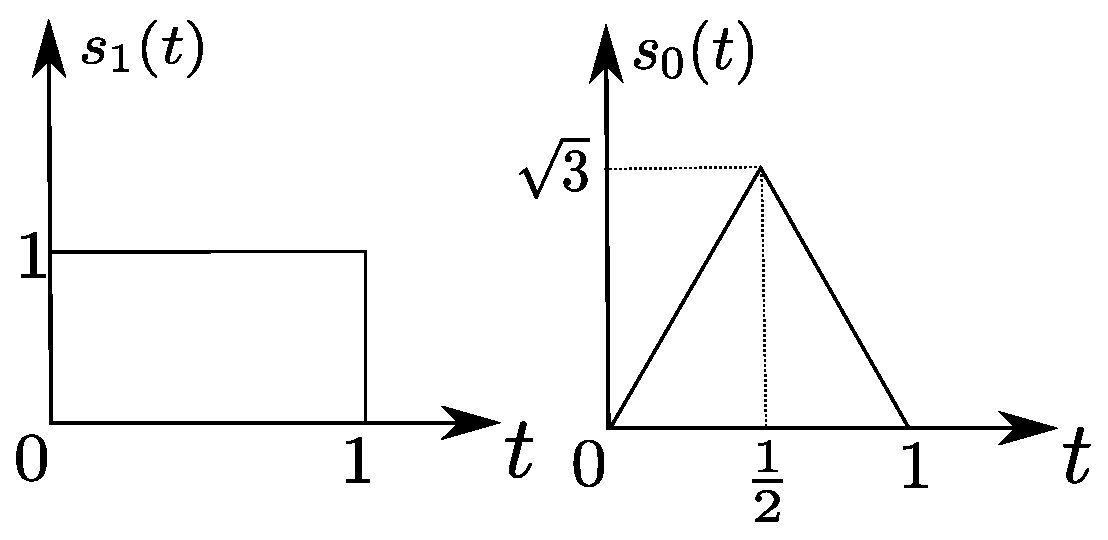
\includegraphics[width=0.7\textwidth]{practice_13.eps}
\caption{信号$s_1(t)$ 和 $s_0(t)$}\label{fig:13}
\end{figure}
\begin{solution}
首先计算信号的能量 $E_1=1,E_2=1,\mathscr{L}_T=1\Rightarrow v_T=0$,根据
\begin{equation}
v \mathop{\gtreqless}^{z\in \mathcal{Z}_1}_{z \in \mathcal{Z}_0} v_T
\end{equation}
可得到最小错误概率的判决准则。
$s_1(t)$和$s_2(t)$的互相关系数$\rho=\frac{\sqrt{3}}{2}$。
由
\begin{equation}\label{eq:continuous_eq_prob}
P_F=P_M=\Phi(-\sqrt{\frac{E(1-\rho)}{N_0}})
\end{equation}
可得到平均错误概率为
$$
\bar{R}=\frac{1}{2}(P_F+P_M)=\Phi\left(-\sqrt{\frac{2E}{N_0}\left(\frac{1}{2}-\frac{\sqrt{3}}{4}\right)}\right)
$$
平均错误概率与$\frac{2E}{N_0}$的函数关系如图\ref{fig:average_error_with_SNR}所示

\begin{figure}[!ht]
\centering
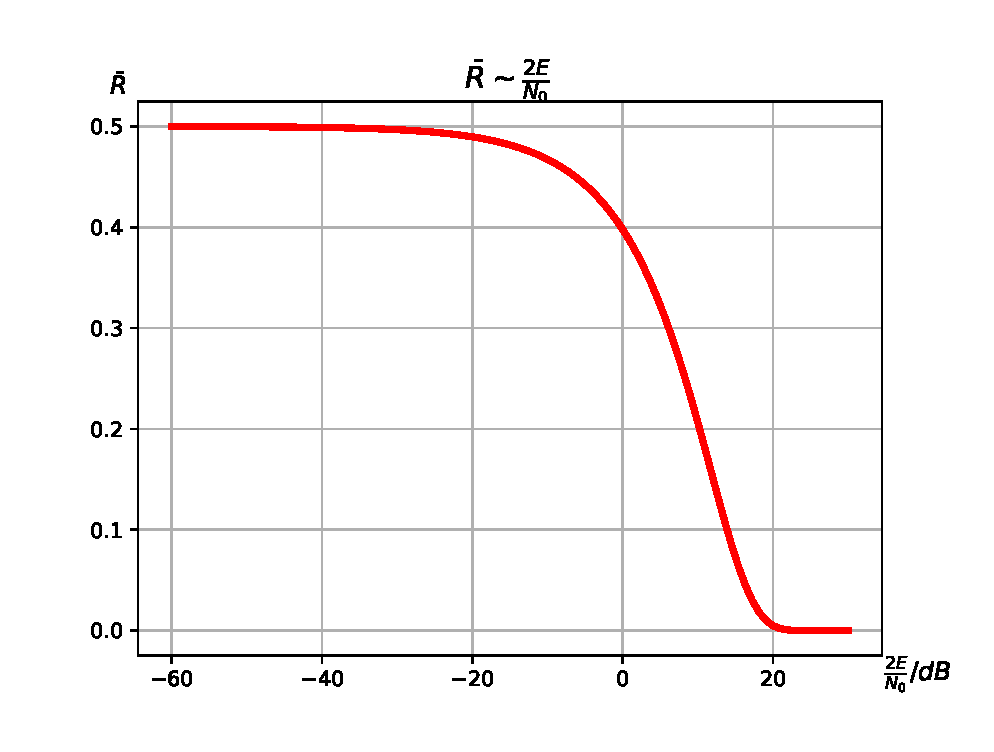
\includegraphics[width=0.7\textwidth]{average_error_with_SNR.eps}
\caption{}\label{fig:average_error_with_SNR}
\end{figure}
\end{solution}
\item 已知$K$个独立的观测值

$\begin{cases}
H_1 : & z_k = n_k \\
H_0 : & z_k = 1 + n_k
\end{cases}$
其中:$n_k$是均值为零、方差为2的高斯随机变量,$k=1,2,\dots,K$。
\begin{enumerate}[label=(\alph*)]
\item 设计似然比检验,并求$P_F$和$P_M$。
\item 画出$K=1$时的接收机工作特性。
\item 假定$c_{00}=c_{11}=0,c_{01}=2,c_{10}=1,P(H_0)=0.7$,试求最小$N$值,使得$K=N$时的风险不大于$K=1$时风险的$\frac{1}{2}$。
\end{enumerate}
\begin{solution}
\begin{enumerate}[label=(\alph*)]
\item 设$\bm{z}=[z_1,\dots,z_K],\lambda(\bm{z})=\frac{p(\bm{z}|H_1)}{p(\bm{z}|H_0)}$
$$
\lambda(\bm{z})\mathop{\gtreqless}_{H_0}^{H_1} \lambda_B \Rightarrow z \mathop{\gtreqless}_{H_1}^{H_0} \frac{1}{2}-\frac{2}{K}\ln \lambda_B
$$
其中$z=\frac{1}{K}\sum_{i=1}^K z_i,z|H_0 \sim N(1,\frac{2}{K}),z|H_1 \sim N(0,\frac{2}{K})$
\begin{align*}
P_F = & \int_{-\infty}^{\frac{1}{2}-\frac{2}{K}\ln \lambda_B} p(z|H_0)dz \\
    = & \Phi\left(-\sqrt{2K}(\frac{1}{4}+\frac{\ln \lambda_B}{K})\right) \\
P_M = & \Phi\left(-\sqrt{2K}(\frac{1}{4}-\frac{\ln \lambda_B}{K})\right)
\end{align*}
\item 当$K=1$时,以$\lambda_B$作为曲线参数,作出$(P_F,P_D)$的曲线如图\ref{fig:ROC_curve} 所示。

\begin{figure}[!ht]
\centering
\includegraphics[width=0.7\textwidth]{ROC_curve.eps}
\caption{}\label{fig:ROC_curve}
\end{figure}

\item 
\begin{align*}
\bar{R} = & C_{01} P(D_0,H_1) + C_{10} P(D_1,H_0) \\
         = & 2 P(H_1) P(D_0 | H_1) + P(H_0) P(D_1 | H_0) \\
         = & 0.6 P_M + 0.7 P_F
\end{align*}
另一方面,
$$
\lambda_B = \frac{P(H_0)(C_{10}-C_{00})}{P(H_1)(C_{01}-C_{11})} = \frac{7}{6}
$$
根据(a)
$\bar{R}(K=1)=0.47,\bar{R}(K=6)=0.25,\bar{R}(K=7)=0.23 < \frac{1}{2}\bar{R}(K=1) \Rightarrow N=7$
\end{enumerate}
\end{solution}
\item 对于二元通信系统,其假设为:

$
\begin{cases}
H_1 : & z(t) = A\cos\omega_1 t + B \cos(\omega_2 t +\phi) + n(t)\\
H_0 : & z(t) = B\cos(\omega_2 t + \phi) + n(t)
\end{cases}
$其中:$\begin{array}{c}
0\leq t \leq T \\
A,B,\omega_1,\omega_2,\phi \textrm{ are known constant}
\end{array}$

假定: $\int_0^T \cos\omega_1 t \cos\omega_2 t dt = \int_0^T \cos\omega_1 t \sin\omega_2 t dt = 0, n(t)$ 是谱密度为$\frac{N_0}{2}$的高斯白噪声。试画出
其最佳接收机模型,并分析其误码率是否和$A\cos\omega_1 t $及$B\cos(\omega_2 t + \phi)$有关。计算误码率以证明你的分析结论。
\begin{solution}
假定等先验概率,由\eqref{eq:continuous_eq_prob}式得 
$$
P_e = \Phi(-\sqrt{\frac{E(1-\rho)}{N_0}})
$$
而
\begin{align*}
E(1-\rho) = & \frac{1}{2} \int_0^T (s_1(t)-s_0(t))^2 dt \\
          = &  \frac{1}{2} \int_0^T (A\cos\omega_1 t)^2 dt 
\end{align*}
因此误码率与$A\cos\omega_1 t$有关而和$B\cos(\omega_2 t + \phi)$无关。
\end{solution}
\end{enumerate}


\end{document}



